\chapter{Methods}\label{ch:methods}
Let us conservatively estimate  how much data is produced when using the LAMP end-station with both pnCCD detectors at a $120$ Hz. Each pnCCD produces 120 images per second, each image is in a 32 bit per pixel format such that an image is vaguely $4$ megabyte in size. So, every minute the front \& rear pnCCD produce approximately $60$ gigabyte of data or 700 gigabyte per 12h shift. To analyze these vasts amount of data an extensive set of methods and optimized algorithms is required. This chapter is devoted to illuminate the analysis methods used in the present thesis.\\
The chapter is organized as follows, Section \ref{sec:LCLS-computing} describes the general LCLS computing environment to establish an overview of the hard- and software capabilities. Section \ref{sec:pnccd-corr} discusses corrections that are applied to the raw pnCCD images.  Section \ref{sec:phase-retrieval} goes over used phase-retrieval algorithms and Section \ref{sec:2d-simulations} discusses simulations of 2D projections of spheres and corresponding diffraction patterns. The Section \ref{sec:acq-considerations}, discusses the Acqiris data acquisition and sampling, while Section \ref{sec:hitfinding} evaluates several hitfinding methods.
%
%
%
\section{The computing environment at LCLS}\label{sec:LCLS-computing}
%%%%%%%%%%%%%%%%
%- Include basics around the PSANA interface\\
%- For example how the date is converted, then stored and\\
%- the analysis opportunities along the way
%- I think this will be a longer subsection since a lot of my work went into this and I'm regularly contacted about it.
%- Short introduction what we have to go through\\
%- Reminder of detectors and analysis environment
%%%%%%%%%%%%%%%%
\begin{figure}
	\centering
		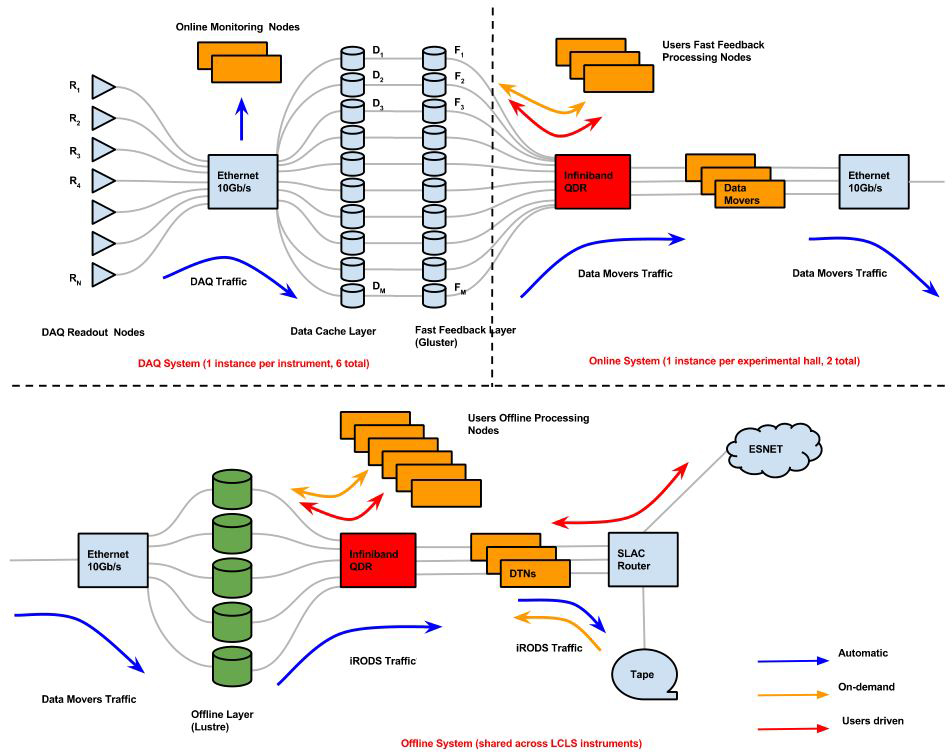
\includegraphics[width=1.00\textwidth]{images/daq-architecture.JPG}
	\caption[Diagram of the computing environment at LCLS and DAQ traffic.]{Diagram of the computing environment at LCLS and DAQ traffic. The recorded data is exchanged through Ethernet and after digitization, is stored on a cache and FFB cluster, where psana computer have access to the online environment during the experiment. Eventually, the data is moved to the more permanent offline environment, where data can be analyzed on psana computers or through a load sharing facility. See more in text. From \citep{Amadeo-2016-SLAC}.}
	\label{fig:daq-architecture}
\end{figure}
As estimated above, the vast amounts of data generated by many detectors are unhandy to handle by a single group of scientists that perform experiments at LCLS. For this reason the LCLS data acquisition (DAQ) group has incorporated many detectors, for example, the pnCCD and Acqiris digitizer into their framework. All data taken at LCLS is stored in the LCLS computing environment, where the data can also be analyzed. As indicated in Figure \ref{fig:daq-architecture}, DAQ readout nodes send the data traffic via Ethernet to a short-term cache and fast feedback (FFB) layer. While the data is being transferred, online monitoring nodes are able to 'see' a fraction of the live (online) data and run analysis. With a delay of a few ten seconds, the FFB nodes can be used to run analysis on the full data stream using parallelization, thereby having 'online' and 'offline' data access. Eventually, the data is being moved to the 'offline' layer, where the data is managed by an integrated Rule-Oriented Data System (iRODS). The data is stored in .XTC file containers and it can also be accessed from outside SLAC (Router \& ESNET). The stored data has certain storage quotas and times. In brief, there is a 6 months short-term storage without quota limitations and a two-year medium-term storage with a storage quota of $10 000$ gigabyte. After that, the data is automatically stored for at least 10 years on magnetic tape (long-term storage) and can be restored upon request. A web interface is provided by the DAQ group to simplify and automate the data-handling and logging process. The short- and medium term storage solutions can also be used to analyze the data using the psana-framework to access data and to perform computations on the psana computer cluster with over 1000 CPU cores. A load sharing facility (LSF) allows the scheduling of (parallelized) batch jobs. The psana-framework can be interacted with python 2.7. The interacting python script calls functions within the psana-framework that are programmed in C(++), for example, detector calibrations. Psana allows parallelization via MPI and it is therefore possible to analyze many events (LCLS pulses) simultaneously. Also complex analysis is able process at the rate of the incoming data using MPI, when the fast feedback buffer (FFB) is used. Python scripts can be written for 'online' or 'offline' analysis and are of similar syntax.\\
For LCLS-II \citep{Amadeo-2016-SLAC}, the analysis and data-access scheme is designed to be similar to Chapter \ref{fig:daq-architecture} with the exception of the online monitoring nodes. It is therefore recommended to build analysis schemes that are based on psana and use the FFB for online analysis, which can then be adapted easily for offline analysis as well. A quick introduction on how to use psana can be found at \url{https://confluence.slac.stanford.edu/display/PSDM/LCLS+Data+Analysis} (from Dezember 2016).
%
%
%
\section{pnCCD photon detectors}\label{sec:pnccd-corr}
%%%%%%%%%%%%%%%%
%- Describe signal on the pnCCDs\\
%- Calibrations and corrections - use LAMP paper\\
%- single hits\\
%- multiple hits
%%%%%%%%%%%%%%%%
\begin{figure}
	\centering
		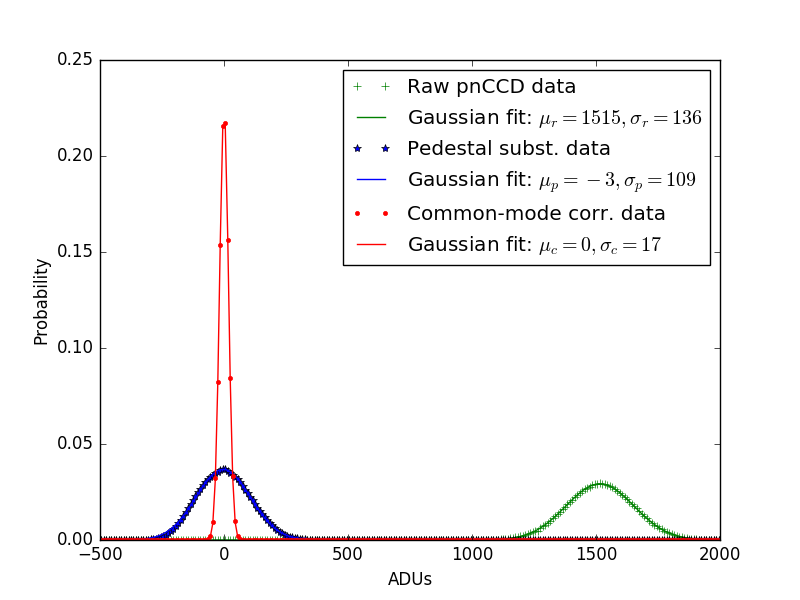
\includegraphics[height=0.50\textwidth]{images/pnCCD-electronic-noise.png}
	\caption[ADU histograms from electronic noise of unilluminated pnCCDs.]{ADU histograms from electronic noise of not illuminated pnCCDs in highest gain mode. The green, plus symbols reflect a histogram of ADU values from raw electronic noise of pnCCD pixel. The noise is set off zero at $\mu_{r}=1515$ ADU and has a standard deviation $\sigma_{r}=136$. The same data shifts to the blue stars after applying a pedestal subtraction. The noise is centered around $\mu_{p}=-3$ and it's standard deviation is reduced to $\sigma_{p}=109$. For the red data points, the common-mode corrections have been applied. Now, the noise is well-centered at $\mu_{c}=0$ ADU and $\sigma_{c}$ is significantly reduced to $17$.}
	\label{fig:pnCCD-electronic-noise}
\end{figure}
Before the pnCCD detectors can be used to take data, it is good practice to apply corrections to the raw detector image in order to cope with electronic noise. Since these corrections are used often, the LCLS detector and DAQ group has implemented a calibration manager tool\index{psana!calibman}\footnote{The calibration manager tool 'calibman' can be found in the 'psana' software package. More information under \url{https://confluence.slac.stanford.edu/display/PSDM/Calibration+Management+Tool} (Oct 2016)} that provides the necessary algorithms and helps with the procedure of applying image corrections and more. We discuss the two most often used corrections next. One, corrects for the electronic noise pedestals\index{pnCCD!pedestal correction} (levels) of each pixel, and two, accounts for common modes\index{pnCCD!common mode}, e.g., artifacts from the read-out electronics that appear for the pnCCD in columns.\\
%
The effects of applying these corrections are illustrated in Chapter \ref{fig:pnCCD-electronic-noise} through a set of histograms. The histogram bins are showing ADU values from dark pnCCD images in highest gain. The green curve shows the ADU values of a raw detector image where no corrections have been applied and the electronic noise response from the chip has a standard deviation of $\sigma_{r}=136$. Note, that there is also a significant offset of the distribution from 0 to $\mu_{r}=1515$ ADU. The blue curve shows the same data but is using the pedestal corrections found in 'calibman'. The pedestal corrections reduce the noise slightly to $\sigma_{p}=109$ ADU, and as expected, the pedestal corrections drastically move the normal distribution to be centered around $\mu_{p}=-3$. Finally, the red curve is also the same data than the green curve but includes pedestal and common-mode corrections. The corrected read-out modes drastically improve the standard deviation to $\sigma_{c}=17$ and slightly move the mean to $\mu_{c}=0$.\\
As a guideline, the pedestal corrections should be always used to account for the mean offset. The common-mode calibration, however, should be tested before applying. The algorithm that determines common-modes needs to find a baseline and therefore needs pixel with no signal in each row and column  \citep{Hantke-Foucard-2016-PC}. In single-particle imaging the detector is illuminated in (almost) every pixel. Then the common-mode correction algorithm may treat real signal as noise and fail to find a common baseline.\\
In the present thesis, pedestal and common-mode correction has always been applied on the front detectors, as these pixel hold mostly signal from single photons. The rear pnCCD uses the pedestal correction but corrects common-modes only above a certain, conservative threshold. See Chapter \ref{fig:pnCCD-image-aligned} for the visible effect on front detector (large, top/bottom arrays) and rear detector (small, centered array).\\
%
%
%
%\subsection{Signal analysis}
%- Present data from 1500eV photon energy on Xe backfilled chamber with the pnCCDs in spectroscopy mode to argue that the pedestal and offset corrections are enough to correct for fluoresence.\\
%- Masked areas in image
%%%
%
%
%
\subsection{Combining multiple pnCCD detectors}\label{sec:combination-of-images}
%%%%%%%%%%%%%%%%%%%%%%%%%
%- Explain how I combined pnCCD detectors to perform reconstructions on it.\\
%- Can reuse material from the LAMP pnCCD paper
%%%%%%%%%%%%%%%%%%%%%%%%%
In order to maximize resolution, it is most useful to combine multiple pnCCD detector modules into one image. While this is a simple task on itself, it becomes more complex, when the combined images need to undergo a phase-retrieval process that use fast Fourier transformations (FFTs). In fact, it has not yet been shown in single-particle imaging that it is possible to retrieve a real space image from multiple detectors in different planes.
%One of the reasons is, that the samples, that were studied in recent years were comparably large, e.g. viral samples of a few hundred nanometer radius that don't scatter to wide angles. Therefore, in many experimental setups, the distance of this detector is then set to fill the detector planes appropriately to the scattering of the sample. In other words, there was no incentive of combining detectors.
The reason for this is that, so far, there was little incentive of merging multiple detectors. Until recently, typical samples were on the order of several hundred nanometers in diameter such that little signal could be detected at large scattering angles. With the intensities provided by LCLS and the single-particle imaging capabilities of the LAMP end-station objects that are smaller than a hundred nanometer in diameter can be studied.
%To cover this variety in object size, LAMP's front pnCCD detector can move along the z-axis and can cover wide scattering angles from smaller objects and LAMP's rear pnCCD detector covers the usual small angles scattering from larger objects. Once the detector is set to cover most scattering angles, one finds that the dynamic range and photon sensitivity becomes a limiting element.
Besides the ability to cover larger scattering angles, multiple detectors can be operated in different gains and still be combined efficiently. For the pnCCD, this allows not only an increase in dynamic range but improves the signal-to-noise.\\
Let us now describe the process of combining diffraction images, while simultaneously preparing them for the inverse problem of phase-retrieval. The discussion now follows the code shown in appendix \ref{sec:combination-of-detectors-code}. The input for the following procedure are two pnCCD images. The images should be pedestal corrected and if possible common-mode corrected. Analysis of the electronic noise determines an cutoff or offset between signal-to-noise for each image (see left Chapter \ref{fig:pnCCD-histogram} and \ref{fig:pnCCD-electronic-noise}). At this step it is also convenient to account for different detector gain settings using the Table \ref{tab:gain-modes} and normalize detector distances using, e.g., the following equation to correct the signal to the front pnCCD plane
\begin{equation}
\text{image}_{\text{normalized}} = \text{image}\cdot \frac{\text{gain}_{\text{front}}}{\text{gain}_{\text{rear}}} \cdot \frac{\text{distance}_{\text{rear}}^{2}}{\text{distance}_{\text{front}}^{2}}
\end{equation}
The pnCCD front top and bottom module are placed in an enlarged array to reflect the real geometry in the plane of the front pnCCD. We can now translate this with a pixel constructed geometry to use the more general scattering angle $\Theta$
\begin{equation}
\Theta = \arctan\left(\frac{\sqrt{\text{pixel}_{\vec{x}}^{2}+\text{pixel}_{\vec{y}}^{2}}\times a}{d}\right),
\label{eqn:scattering-angle}
\end{equation}
with $pixel_{\vec{x}}$ and $pixel_{\vec{y}}$ being the length of the pixel array from the beam along the X- and Y-axis, respectively. We can use this information to further generalize the matter and attribute a scattering vector $\vec{Q}$ to each pixel
\begin{equation}
\vec{Q} = 4 \pi \frac{\sin\left(\frac{\Theta}{2}\right)}{\lambda},
\label{eqn:q-vector}
\end{equation}
with $\lambda$ being the wavelength of the scattered photons. We can now add the signal from the rear pnCCD to the enlarged array, while using the generalized coordinates $\vec{Q}$. In this generalized downsampling process, the arithmetic mean of the downsampled pixel is used, which is why a normalization factor needs to be carried. The downsampling into the enlarged array also  preserves the pixel size of the front pnCCD (enlarged) array and allows Fast Fourier Transformation (FFT) algorithms to use the array. The usage of FFT algorithms is of great interest to reduce computing times in iterative phase-retrieval algorithms.\\
%
%
%
\begin{figure}
	\centering
		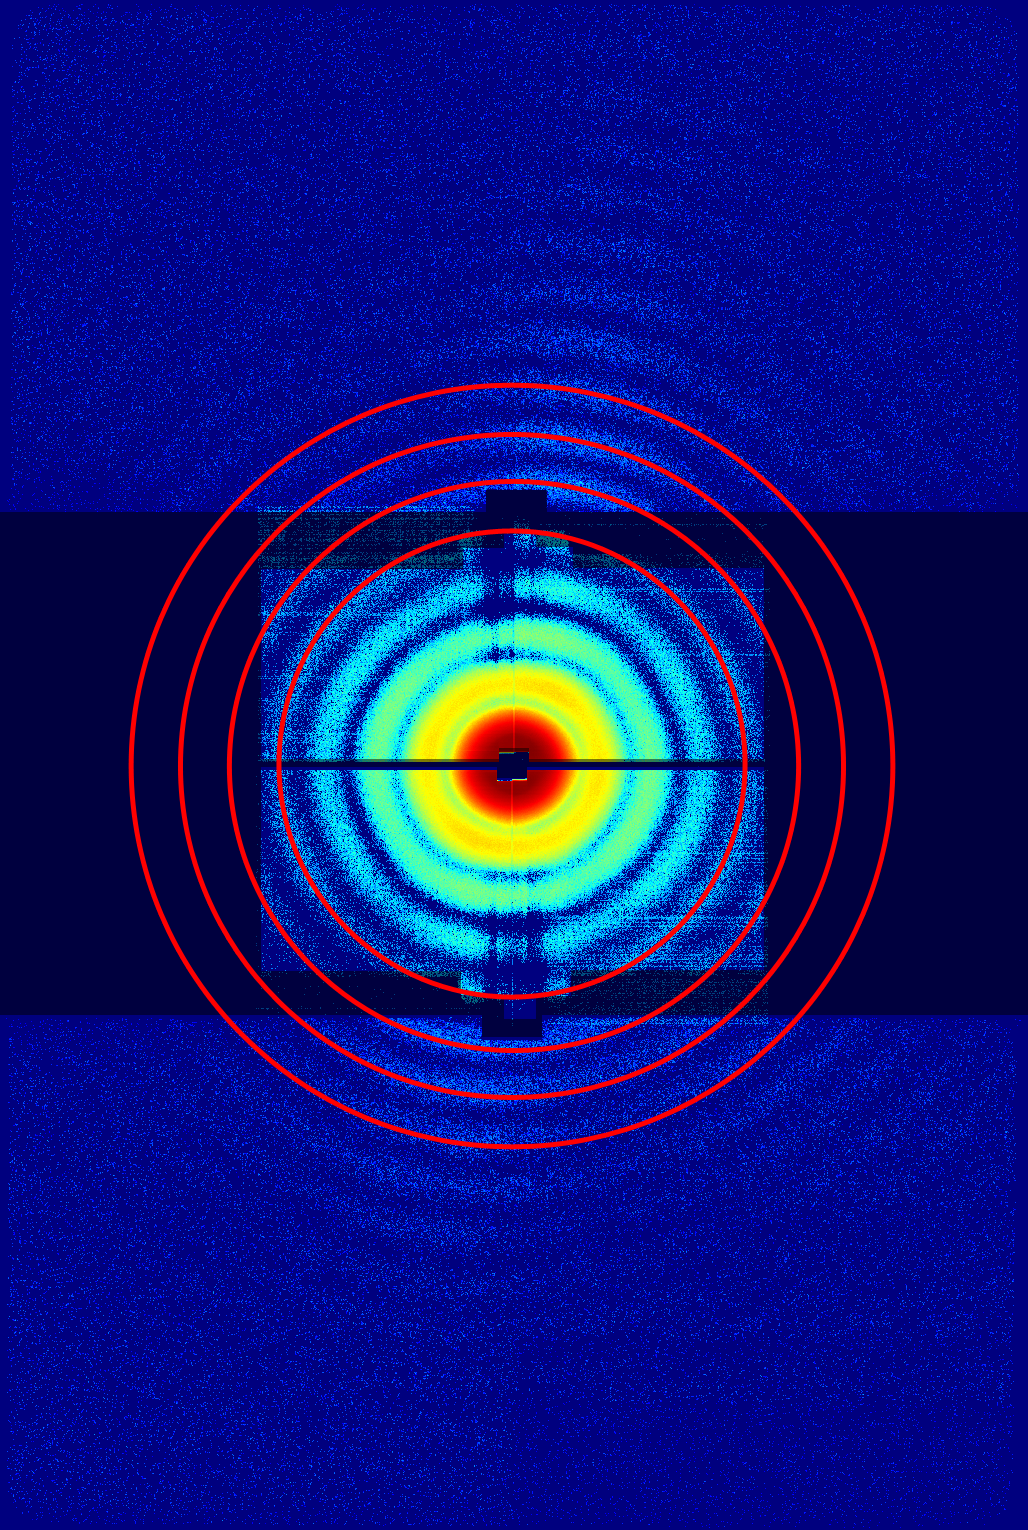
\includegraphics[width=0.8\textwidth]{images/pnCCD-image-geometry.png}
	\caption[Front and rear pnCCD arranged to combine measured diffraction image.]{A combined pnCCD image using the full image of the front pnCCD and a down-sampled image of the rear pnCCD. The red circles in the image are drawn to visualize the alignment of the detectors. As described in the text, the intensities in the image are normalized and corrected for different electronic gains and distance to specific detectors. The shaded areas are not covered by the pnCCDs and are therefore masked out.}
	\label{fig:pnCCD-image-aligned}
\end{figure}
Figure \ref{fig:pnCCD-image-aligned}a shows a diffraction pattern from a spherical xenon cluster of $\sim 50$ nm in radius. The front pnCCD detector was set to slightly overlap with the rear pnCCD detector along the Y-axis but the front detector was set $\sim 365$ mm closer to the interaction region along the Z-axis. All four of LAMP's pnCCD modules have been combined in one image, and since the rear pnCCD is farther away from the interaction region it appears smaller on the combined image. The red circles are a help for the eye to align the modules and show how the diffraction pattern overlaps. In this case, the front pnCCD was operated in highest gain $\frac{1}{1}$ and the rear pnCCD was operated in lowest gain $\frac{1}{256}$.\\
\begin{figure}
	\centering
		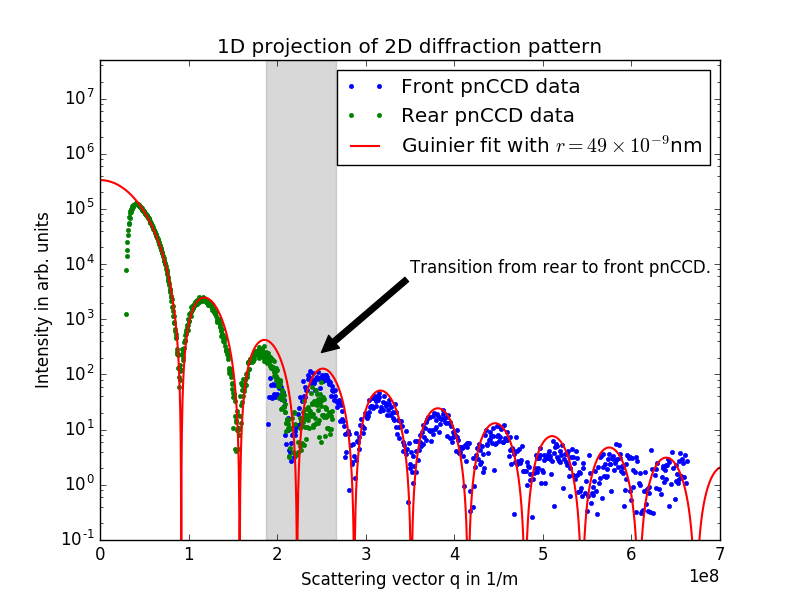
\includegraphics[height=0.50\textwidth]{images/pnCCD-1d-sum.png}
	\caption[Spherical projection of 2D diffraction image onto 1D.]{Spherical projection of 2D diffraction image onto 1D. The data points are from the rear pnCCD (green points) and the front pnCCD (blue points) have been combined. The gray shaded area shows the transition area from rear to front detector. The red curve is a simulated scattering curve from an ideal sphere (see Equation \eqref{eq:scattering from sphere}). The amplitude of the red curve has been fitted to the data points and it agrees well with the data.}
	\label{fig:pnCCD-1d-sum}
\end{figure}
The radial intensity profile yields valuable information about the geometric alignment and intensity normalization. Figure \ref{fig:pnCCD-1d-sum} shows the radial intensity profile of the spherical symmetric diffraction image over 5 orders of magnitude above the noise level. The red curve illustrates the expected scattering intensity of a spherical object using Equation \eqref{eq:scattered-intensity} and \eqref{eq:scattering from sphere}. An automated fitting routine determined the radius $r$ of the cluster, here, $r=49$ nm and the incident beam intensity $I_{0}$, which was determined based on zero order scattering. The curve showcases the validity of the detected signal up to the edges of the front pnCCD, where little signal is present. There are also some discrepancies from the red curve on the transition from the rear to front pnCCD, which are due to the shade projected from the front onto the rear pnCCD and the resulting lack of signal.
%
%
%
\subsection{Impact of the X-ray pump--X-ray probe on diffraction pattern}\label{sec:pump--probe-considerations}
\begin{figure}
	\centering
		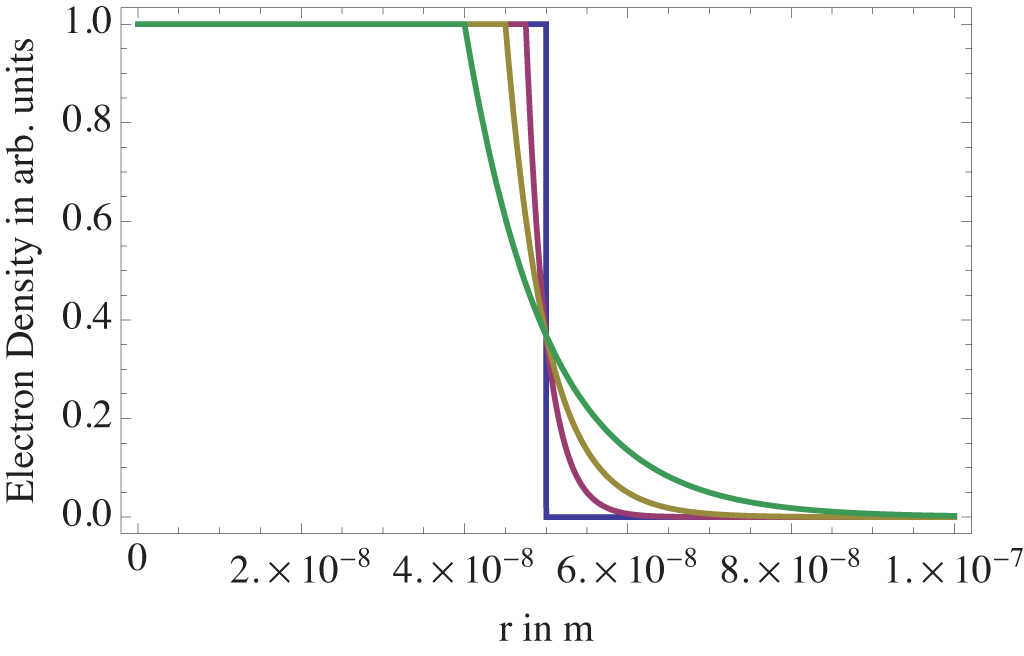
\includegraphics[width=0.49\textwidth]{images/electron-density-convoluted-object.png}
		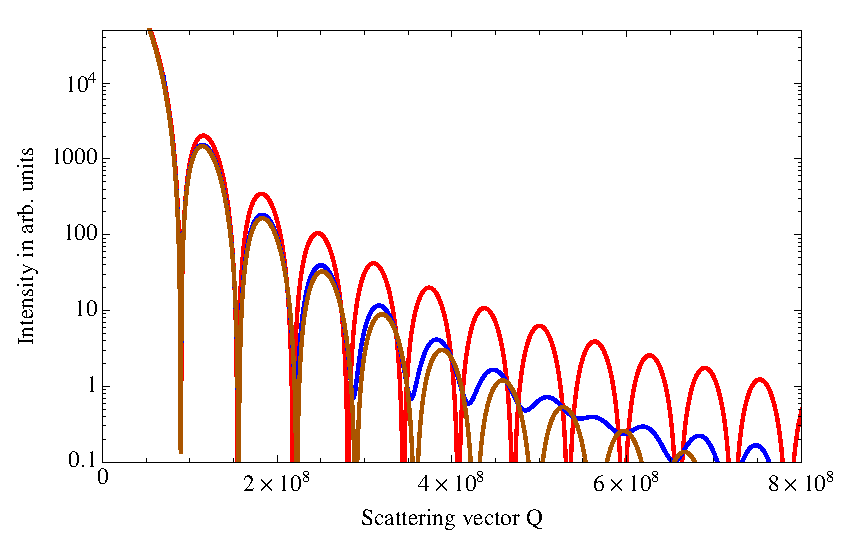
\includegraphics[width=0.49\textwidth]{images/beam-convoluted-with-object.eps}
	\caption[Influence of X-ray pump--X-ray probe study in diffraction image.]{Left: electron density of an expanding spherical symmetric nanoplasma. Right: red line, scattering of an intact sphere. Brown, scattering of an expanding sphere with $k=5$ nm. Blue, combined scattering of an intact and expanding sphere that has been pumped with $10\%$- and probed with $90\%$ of the overall pulse energy. See more information in text.}
	\label{fig:electron-density-convoluted-object}
\end{figure}
In a coherent diffractive imaging X-ray pump--X-ray probe experiment, both pulses contribute to the scattering image. The pump-pulse will project an image of the solid and intact cluster, while the probe-pulse will propagate an image of the expanding, damaged cluster. In the present experiment, the pump-pulse was set at $\sim10\%$ of the overall pulse energy, while the probe-pulse was set to $\sim90\%$ of the overall pulse energy. In order to simulate the effects of the X-ray pump-- X-ray probe setup, a 1D simulation is conducted using electron densities $\rho\left(r\right)$ of spheres. Although rare-gas cluster exhibit an icosahedral structure, at present resolution cluster can be well simulated using spheres. The spheres are allowed to expand after the model
\begin{align}
\rho\left(r, k\right)&=\begin{cases}
1& \text{for $R-k \geq r \geq 0$},\\
e^{\frac{(R-k)-r}{k}}&\text{for $R > r - k$},
\end{cases}
\intertext{with $R$ being the cluster radius and $k$ an expansion coefficient such that}
\int_{0}^{\infty}\rho\left(r, k\right)dr &= R,\quad \text{if } 0<k<R 
\label{eq:el-density-expanding}
\end{align}
The electron density can then be Fourier transformed into recipocal space using the transformation \citep{Guinier-1955-JWS}
\begin{equation}
I\left(\vec{Q}\right)=I_{0}F^{2}(Q)=I_{0} \left(\int_{0}^{\infty}\rho\left(r,k\right)\frac{\sin\left(Q r\right)}{Qr}4 \pi r^{2}dr\right)^{2},
\label{eq:guinier-fourier-transform}
\end{equation}
with $I_{0}$ being an intensity scaling factor. The electron densities for $R=50$ nm and $k=\{0,2.5,5,10\}$ nm are shown in Chapter \ref{fig:electron-density-convoluted-object} left. Figure \ref{fig:electron-density-convoluted-object} right showcases several cases of (expanding) spheres in reciprocal space. The red line is the scattering of a solid sphere $F_{\text{intact}}^{2}$, with $A$ being used to scale the intensity to typical experimental data. The brown curve is the scattering of an expanding sphere $F_{\text{expanding}}^{2}$ with $R=50$ nm and $k=5$ nm. Lastly, the blue curve corresponds to the case, where $A\cdot F^{2}\rightarrow A \cdot 10\% F_{\text{intact}}^{2}+A \cdot 90\% F_{\text{expanding}}^{2}$. Although the pump-pulse influences the diffraction pattern visibly at high-Q values, the added signal remains in the noise level of $F^{2}(Q)<1$ (compare Chapter \ref{fig:pnCCD-1d-sum}).
%
%
%
\section{Phase retrieval from a single diffraction pattern}\label{sec:phase-retrieval}
%%%%%%%%%%%%%%
%- Short intro into phase retrieval
%%%%%%%%%%%%%%
As deducted in Section \ref{sec:saxs}, coherent diffractive imaging merely measures the intensity in reciprocal space and the phase information, i.e., complex fields are lost. Iterative algorithms can retrieve this lost information because there are only limited sets of phases that uniquely reproduce the diffraction image \citep{Bruck-1979-OpticsCom,Bates-1981-Optik}. To fully recover the original function, i.e., real and complex values of the diffraction pattern, the diffraction image must be oversampled\index{oversampling} \citep{Sayre-1952-ActCryst}. Here, the Nyquist-Shannon sampling\index{oversampling!Nyquist-Shannon sampling theorem} theorem says that a Fourier transformed object of size $X$ can be fully recovered if its sampling rate is at the Nyquist rate\index{oversampling!Nyquist rate} of $\frac{1}{2X}$\index{}. The Nyquist rate can be translated into a minimum (pnCCD) pixelsize in realspace using the following relation between a discrete Fourier transform and pixel length $\Delta_{r}$ \citep{Williams-2010-NJP}
\begin{equation}
\Delta_{r} = \frac{\lambda L}{2 X},
\label{eq:disc-fourier-relation-pixelsize}
\end{equation}
with the wavelength $\lambda$, the length to the detector $L$ and the object length along one dimension $X$. For typical experimental values, the sampling pixel size must be $\Delta_{r} \leq 2.7$ mm along all pixel dimension to fully recover the particle's (projected) electron density. In the present experiment, the pnCCD pixel size of $75 \times 75~\mu\text{m}^{2}$ samples the object sufficiently enough. And this still holds true for the downsampled pixel in the combined pnCCD images.
%
%
%
\subsection{Principle of phase retrieval}\label{sec:phase-retrieval-fundamental}
%%%%%%%%%%%%%%
%- Introduce some aspects from phase retrieval algorithms.
%%%%%%%%%%%%%%
\begin{figure}
	\centering
		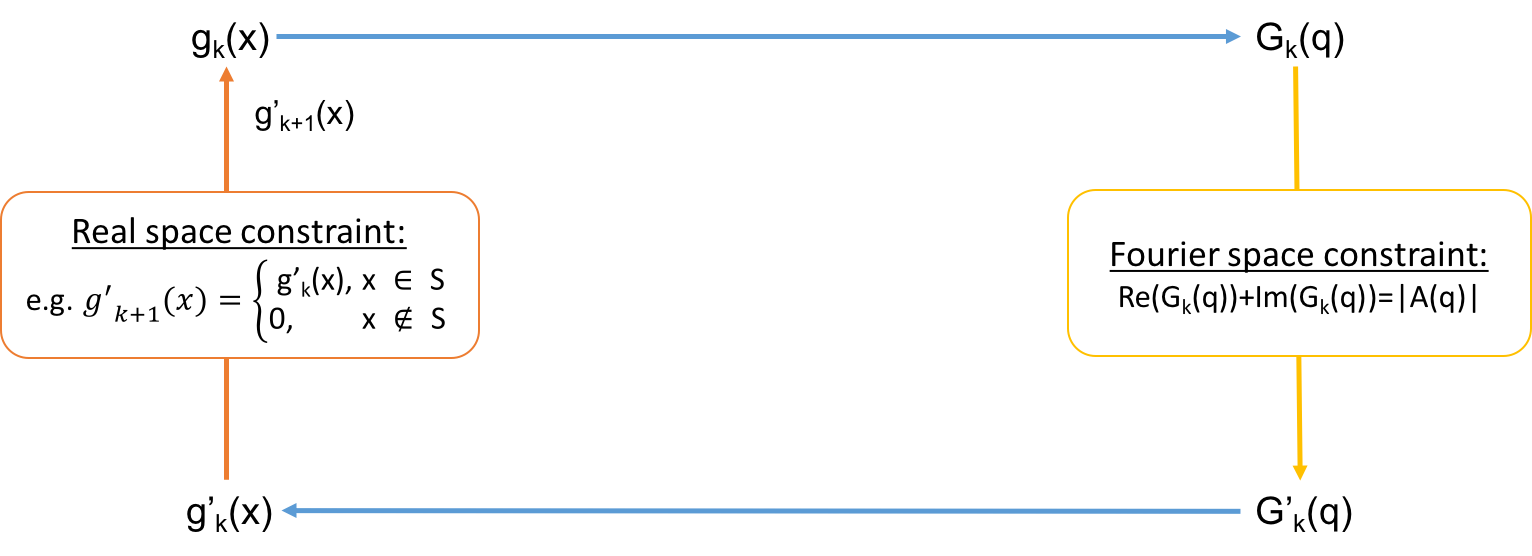
\includegraphics[width=0.80\textwidth]{images/phase-retrieval-algorithm.png}
	\caption[Example of a phase retrieval algorithm.]{Principle of a phase retrieval algorithm. The real space object $g_{k}\left(x\right)$ is Fourier transformed to $G_{k}\left(q\right)$. The function $G_{k}\left(q\right)$ is altered to fit the constraints set in Fourier space and becomes $G'_{k}\left(q\right)$. $G'_{k}\left(q\right)$ is inverse Fourier transformed to $g'_{k}\left(x\right)$. After fulfilling the real space constraints the iterative starts again using $g_{k+1}\left(x\right)$. After \citep{Fienup-1982-AO}.}
	\label{fig:phase-retrieval-algorithm}
\end{figure}
To recover the phase from an oversampled diffraction pattern and thus reconstruct an image of the object, iterative algorithms have been developed \cite{Fienup-1982-AO}. Figure \ref{fig:phase-retrieval-algorithm} illustrates such an iterative algorithm, where the image of an object $g_{k}\left(x\right)$ is Fourier transformed to reciprocal space $G_{k}\left(x\right)$ and then back again resulting in $g_{k+1}(x)$, while sufficing certain constraints.\\
The constraints are rather strict defined in the reciprocal space as they have to reproduce the actual measurement $I=A\cdot A^{*}$, which is sometimes called the modulo constraint. The criteria that need to be met in real space can be chosen more freely. Generally, the recovered object should be physical, i.e., should be of a certain (known) size. One can introduce a support structure $S$ that meets the physical constraints and can therefore be used to, for example, zero outlying values. Throughout the iterations, the functions $g_{k}(x)$ evolve and eventually converge into a solution. If one uses the above criterion, one can show that the error between the reconstructions and the actual measurement continuously reduces, which is why it is commonly referred to as error-reduction algorithm \cite{Fienup-1978-OL}.
%
%
%
%
%\subsection{Solving the inverse problem}
\subsection{2D reconstructions and image resolution}
%
%
%
\subsubsection{Hawk program for 2D image phase retrieval}
%%%%%%%%%%%%%%%%%
%- Describe Filipe's program
%%%%%%%%%%%%%%%%%
For all image reconstructions in 2D, the Hawk software package\index{Hawk software package} \citep{Maia-2010-JAC} has been used. Hawk is available under the GNU General Public License\footnote{Hawk copyright: \url{https://github.com/FXIhub/hawk/blob/master/Copyright}} and can be downloaded with installation instructions from \url{https://github.com/FXIhub/hawk}. In previous efforts to retrieve a real-space image from FEL based coherent diffractive imaging, Hawk has been used successfully in several reconstructions ranging from viruses \citep{Seibert-2011-Nature,Ekeberg-2015-PRL} to other few hundred nanometer sized objects \citep{Seibert-2010-JPhysB} but has not yet been used to recover the realspace image from rare-gas cluster.
\begin{table}%[h!]
\centering
\begin{tabular}{ |c|c|}
 \hline
 \textbf{Parameter} & \textbf{Setting} \\ 
 %a & b & c & d & e \\
 %[0.5ex] 
 \hline
 Starting Guess & random phases \\ \hline
 Autocorrelation Selection & threshold \\ \hline
 Autocorrelaton Threshold & 0.04  \\ \hline
 Phasing method beta & 0.9  \\ \hline
 Beta range & 0 - $\infty$ \\ \hline
 Enforce positivity & false   \\ \hline
 Enforce real & false     \\\hline
Perturb weak reflections & false \\ \hline
Phasing algorithm & raar \\ \hline
Blur & 12 - 0.7 \\ \hline
Blur range & 0 - 12000 \\ \hline
Center image & false \\ \hline
Object area & 0.0022 - 0.0019 \\ \hline
Object area range & 0-8000\\ \hline
Support update algorithm & area \\ \hline
\end{tabular}
\caption[Typical parameters used in the Hawk software package.]{Typical parameters used in the Hawk software package. The object area depends strongly on the actual particle size and thus varies.}
\label{tab:hawk-parameter}
\end{table}
The usage of the program is straight forward in three steps. First, the diffraction images are transformed into the '.cxi' format \citep{Maia-2012-NatMet}. Second, diffraction images are prepared in \textit{Hawk's editor}, where particular effort has to be made to create a proper mask. The mask  allows to forgo saturated, shadowed or otherwise faulty pixel. The software suite automatically interpolates between masked pixel. The successful edited '.cxi' file is then saved in Hawk's '.h5' format. Third, \textit{Hawk's phaser} can be used to iteratively retrieve the phase from the '.h5' intensity file. Typical parameter for the phaser can be found in Table \ref{tab:hawk-parameter}. Here the \textit{RAAR algorithm} \cite{Luke-2005-IP} in combination with initially strong \textit{blurs}, the extension of the \textit{phasing beta range} and a proper determination of the \textit{object area} (support structure size) resulted in useful reconstructions. Note, that the \textit{object area} size differs from particle to particle and is a sensitive parameter. After $10^{5}$ to $1.5\cdot 10^{5}$ iterations, the real space object typically converges.
%
%
%
\subsubsection{Resolution enhancement through combination of rear and front pnCCD}\label{sec:resolution-discussion}
%%%%%%%%%%%%%%%
%- Showcase difference of rear pnCCD only vs. front + rear pnCCD vs. front + rear pnCCD 'cropped' for best results. Recycle work from LAMP pnCCD paper
%%%%%%%%%%%%%%%
\begin{figure}
  \begin{center}
   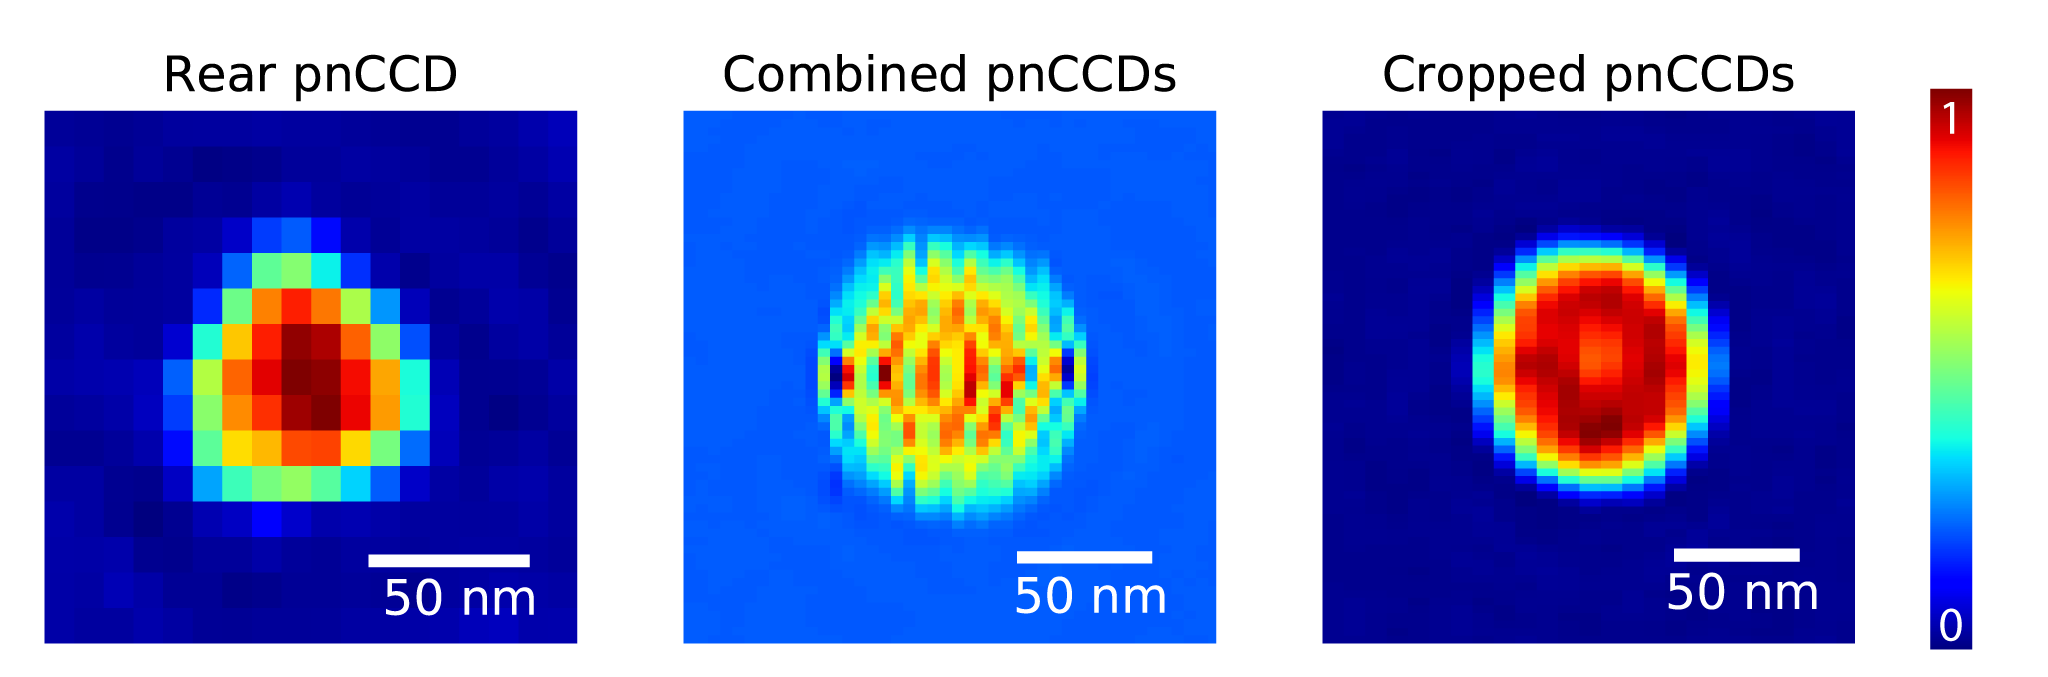
\includegraphics[width=0.8\linewidth]{images/Phase-retrieval-image.png}\\
   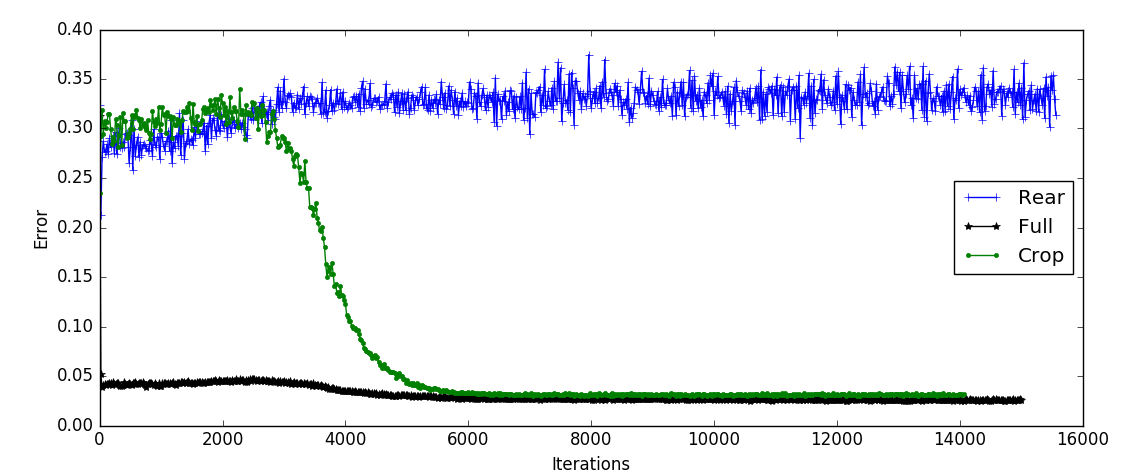
\includegraphics[height=3.5cm]{images/Phase-retrieval-error.png}
    \caption[Illustration of resolution enhancement and diffraction image cropping.]{Illustration of resolution enhancement due to detector combination. The diffraction pattern in Chapter \ref{fig:pnCCD-image-aligned} of a Xe-cluster has been reconstructed to illustrate several cases. Top left: Rear pnCCD data only reconstruction yields a non-spherical object; error criterion shows no convergence (see graph). Top middle: Front \& rear pnCCD data results in a spherical object but missing areas next to the rear pnCCD disturb the reconstruction process, such that the electron density becomes unphysical. Top right: A cropped diffraction image without the missing areas next to rear pnCCD enables a physical reconstruction.}
\label{fig:phase-retrieval-image}
  \end{center}
\end{figure}
While there is no consensus on how to define resolution in a coherent diffractive imaging pattern and the resulting reconstruction there are various good estimates. A simple and conservative method to define resolution in a diffraction pattern is Abbe's criterion, which comes from microscopy and calculates the minimal resolvable feature size in a diffraction pattern. The fundamental limit that the minimal resolvable feature size is dependent on the wavelength has also given us the inspiration to build short-wavelength machines such as the free electron laser and synchrotron light sources.\\
First, we must verify that we are in the far field by fulfilling the following requirement \cite{Williams-2010-NJP}
\begin{equation}
\frac{d^{2}}{\lambda L} \ll 1
\label{eq:far-field-test}
\end{equation}
with the wavelength of the X-rays $\lambda$, the distance to the detector $L$ and the object size $d$. In this experiment, the criterion is met.\\
In the far field, Abbe's criterion can be written down as
% Internal note, Max did check that we are in the far field.
\begin{equation}
    d = \frac{\lambda}{2n \sin(\frac{\Theta}{2})},
		\label{eq:abbe-criterion}
\end{equation}
with the minimal resolvable feature size $d$, the refractive index $n$ and the half scattering angle $\frac{\Theta}{2}$. The scattering angle is restricted by either the active detector area, which goes back to the typical understanding of a numerical aperture, or the signal intensity up to certain angles. The latter is in interplay with the photon wavelength and object cross-sections. This interplay leads to the current assessment that very high energy photons, e.g., $8$ keV photons that are commonly used for crystallographic purposes, scatter too little signal. Additionally, low-$\vec{Q}$ scattering is often unresolvable due to straylight. As current results indicate, using $0.5-5$ keV photons ultimately lead to higher resolution images than using $8$ keV photons \citep{Aquila-2015-StrucDyn}.\\
In the far field, we can use the following equation to investigate the pixel size \cite{Williams-2010-NJP}
\begin{equation}
    \Delta_{s} = \frac{\lambda L}{N \Delta_{d}},
\label{eq:relation-pixel-fourier}
\end{equation}
with $L$ being the length from the interaction region to the detector, $\Delta_{i}$ being the linear pixel size that is linked to each other through the discrete Fourier transformation and $N$ being the side length of the discrete detector array.\\
Figure \ref{fig:phase-retrieval-image} top shows several reconstructions of xenon cluster at $\lambda = 1.0$ nm using different snippets of the diffraction pattern in Chapter \ref{fig:pnCCD-image-aligned}. If just the rear pnCCD is used for reconstructions, a maximum scattering angle of $\Theta\approx 4.2$° is recorded, which results in a minimal resolvable feature size of $d\approx 14$ nm. However, in the present data a shadow is cast on the CCD reducing the maximum scattering angle in the image \textbf{'Rear pnCCD'} to $\Theta\approx 3.8$° and thus the resolution to $d\approx 15$ nm. The pixel size is $\sim 10 \text{nm} \times \sim 12 \text{nm}$. The image \textbf{'Combined pnCCDs'} uses the whole data including the empty areas next to the rear pnCCD. The image shows an unphysical electron density distribution, which origins from the empty areas next to the rear pnCCD data. In these areas, the interpolation along the Y-axis/ extrapolation along the X-axis fails. The next image \textbf{'Cropped pnCCDs'} uses data in full extend along the Y-axis but is cropped along the X-axis such that the blank areas are excluded. The reconstruction converges into an object that appears physical. The maximum scattering angle here is $\Theta \approx 9.2$° and the resolution thus $d\approx 6$ nm. The pixel size here is $\sim 10 \text{nm} \times \sim 3 \text{nm}$.\\
This is a factor $\sim 5$ improvement over common cited studies in single particle imaging \citep{Seibert-2011-Nature} and still a factor $\sim 3$ better than \citep{Hantke-2014-NatPho}, where measured diffraction patterns have been 'computationally purified'. The resolution enhancement due to the combination of detectors can be abused further using EMC algorithms \citep{Loh-2009-PRE}, where multiple images can be arranged due to their rotation and averaged, hence filling the missing areas next to the rear pnCCDs and allowing 3D reconstructions with (few\footnote{Depending on the position of the front pnCCD.}) nanometer resolution.\\
%
%
%
\subsection{1D projections and phase reconstructions}\label{sec:1d-proj-and-phase-reconstruction}
%%%%%%%%%%%%%%%%
%- Describe my algorithm in 1D in detail
%%%%%%%%%%%%%%%%
To display many effects in diffraction pattern, they have sometimes been reduced from two dimensions to merely one. A 1D representation of the data allows easy to interpret comparison to analytical models. To reduce the 2D diffraction data to 1D the program shown in appendix \ref{sec:spherical-integration} has been employed. It is based on Matlab\index{Matlab} to efficiently iterate through pixel arrays. The input for this program are pedestal calibrated diffraction images that have unwanted areas masked out and a true image center defined. Key elements of the algorithm are to iterate through every pixel, filtering signal from noise, determining the $\vec{Q}$-value of every pixel and sum signal over $\vec{Q}$, while normalizing the data over pixel. Additionally, an algorithm has been designed to perform phase retrieval on the 1D data.
%This program is based on python and can also be found in appendix \ref{sec:1d-phase-retrieval-code}. The input for this algorithm are mirrored, zero-frequency (inverse) shifted 1D diffraction arrays.
The algorithm follows the fundamental scheme described in sub-Section \ref{sec:phase-retrieval-fundamental}. Thereby, the realspace data of the object is forced to be real and positive, which is also the error criterion in real space. The difference to the measured data yields the error criterion in Fourier space. The algorithm allows monitoring of the Fourier- and realspace error, the phase and the actual Fourier and realspace images. The iterative algorithm is aborted based on the error criterion.
%
%
%
\section{2D electron density and diffraction image simulations}\label{sec:2d-simulations}
%%%%%%%%%%%%%%%%%%%%%%%%%%%
% Describe 2D simulations
%%%%%%%%%%%%%%%%%%%%%%%%%%%
\begin{figure}
	\centering
		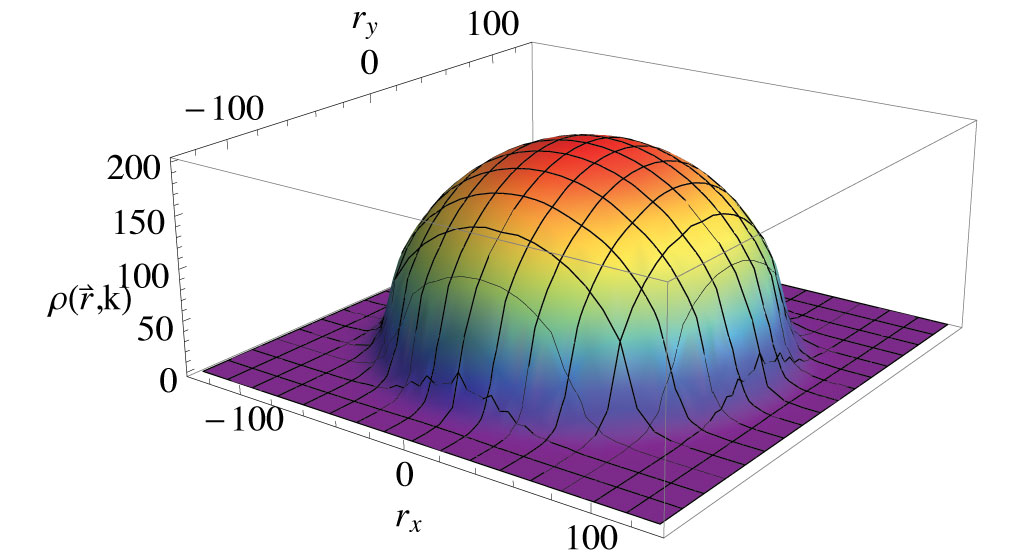
\includegraphics[width=0.49\textwidth]{images/cluster-generation-2D.jpg}
		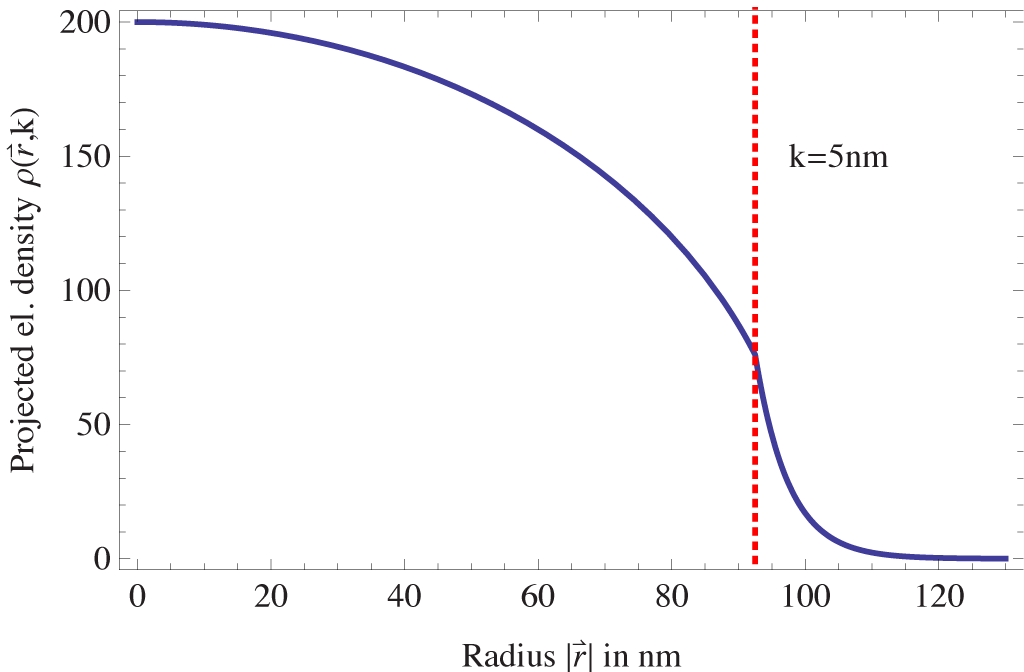
\includegraphics[width=0.49\textwidth]{images/cluster-generation-1D.png}
	\caption[Used electron densities in 2D real and Fourier space simulations.]{Left: Electron density of a $R\approx 100nm$ expanding sphere with $k=5$ nm, projected onto a 2D plane. Right: Blue curve, spherical projection of the 2D simulation to 1D. Red dashed line, point of expanding density at $k=5$ nm.}
	\label{fig:cluster-generation}
\end{figure}
The interpretation of the helium cluster doped with xenon data requires a more thorough investigation than with 1D fits possible. Therefore two dimensional studies were performed to simulate electron densities of (doped) clusters. The electron density is then Fourier transformed to yield 2D diffraction images, which can be compared to the experimental data. The 2D simulations can then optionally be reduced to 1D using a spherical integration (see subSection \ref{sec:1d-proj-and-phase-reconstruction}) to be easily compared to the experimental data and other analytical models. The clusters are approximated using spheres, which is at the current resolution an acceptable estimation of the icosahedral cluster structure. In the simulated cluster, i.e., core-shell system, the shell consists of one large cluster with low electron density (helium) and the core comprises smaller dense spheres (xenon) at different locations within the shell. Furthermore, the spheres can expand to simulate the effect of a nanoplasma expansion. We can express such spheres using the formalism
\begin{align}
\rho_{i}\left(\vec{r}, k\right)&=\begin{cases}
2 \sqrt{R^{2}-\left|\vec{r}\right|^{2}} \cdot \rho_{0}& \text{for $R-\frac{3 k}{2} \geq \left|\vec{r}\right| \geq 0$},\\
2 \sqrt{R^{2}-\left|\vec{r}\right|^{2}} \cdot \rho_{0} e^{\frac{(R-\frac{3k}{2})-\left|\vec{r}\right|}{k}}&\text{for $R > \left|\vec{r}\right| - \frac{3k}{2}$},
\end{cases}
\label{eq:el-density-expanding-2d}
\intertext{with $\rho_{0}$ being the density, $R$ being the cluster radius and $k$ an expansion coefficient such that}
\int_{0}^{\infty}\rho\left(\left|\vec{r}\right|, k\right)d\vec{r} &= R,\quad \text{if } 0<k<R 
\end{align}
Multiple spheres $\rho_{i}\left(\vec{r}\right)$, with $i=1,2,3,...$, can be positioned using $\vec{r}\rightarrow \vec{r}-\vec{r_{0}}$, with $\vec{r_{0}}$ being the center of mass of the sphere $\rho_{i}$. The density $\rho_{0}$ was set to $\rho_{0, \text{helium}}=1$ for liquid helium and $\rho_{0,\text{xenon}}=\frac{3.640}{0.1412}\approx 25.8$ for xenon. The numerator of the fraction for $\rho_{0,\text{xenon}}$ is the density of bulk xenon\index{Xenon!bulk density} in g/cm$^{3}$ and the denominator is the density for liquid helium\index{Helium!liquid density} in g/cm$^{3}$. Using Equation \eqref{eq:el-density-expanding-2d}, a large array of $\sim 1500\times 1500$ is generated that is comparable to the combined pnCCD image array size. The array is then Fourier transformed\index{Fourier Transform} using Matlab's\index{Matlab} \textit{fft2} and the output is subsequently rearranged using \textit{fftshift}.\\
\begin{figure}
	\centering
		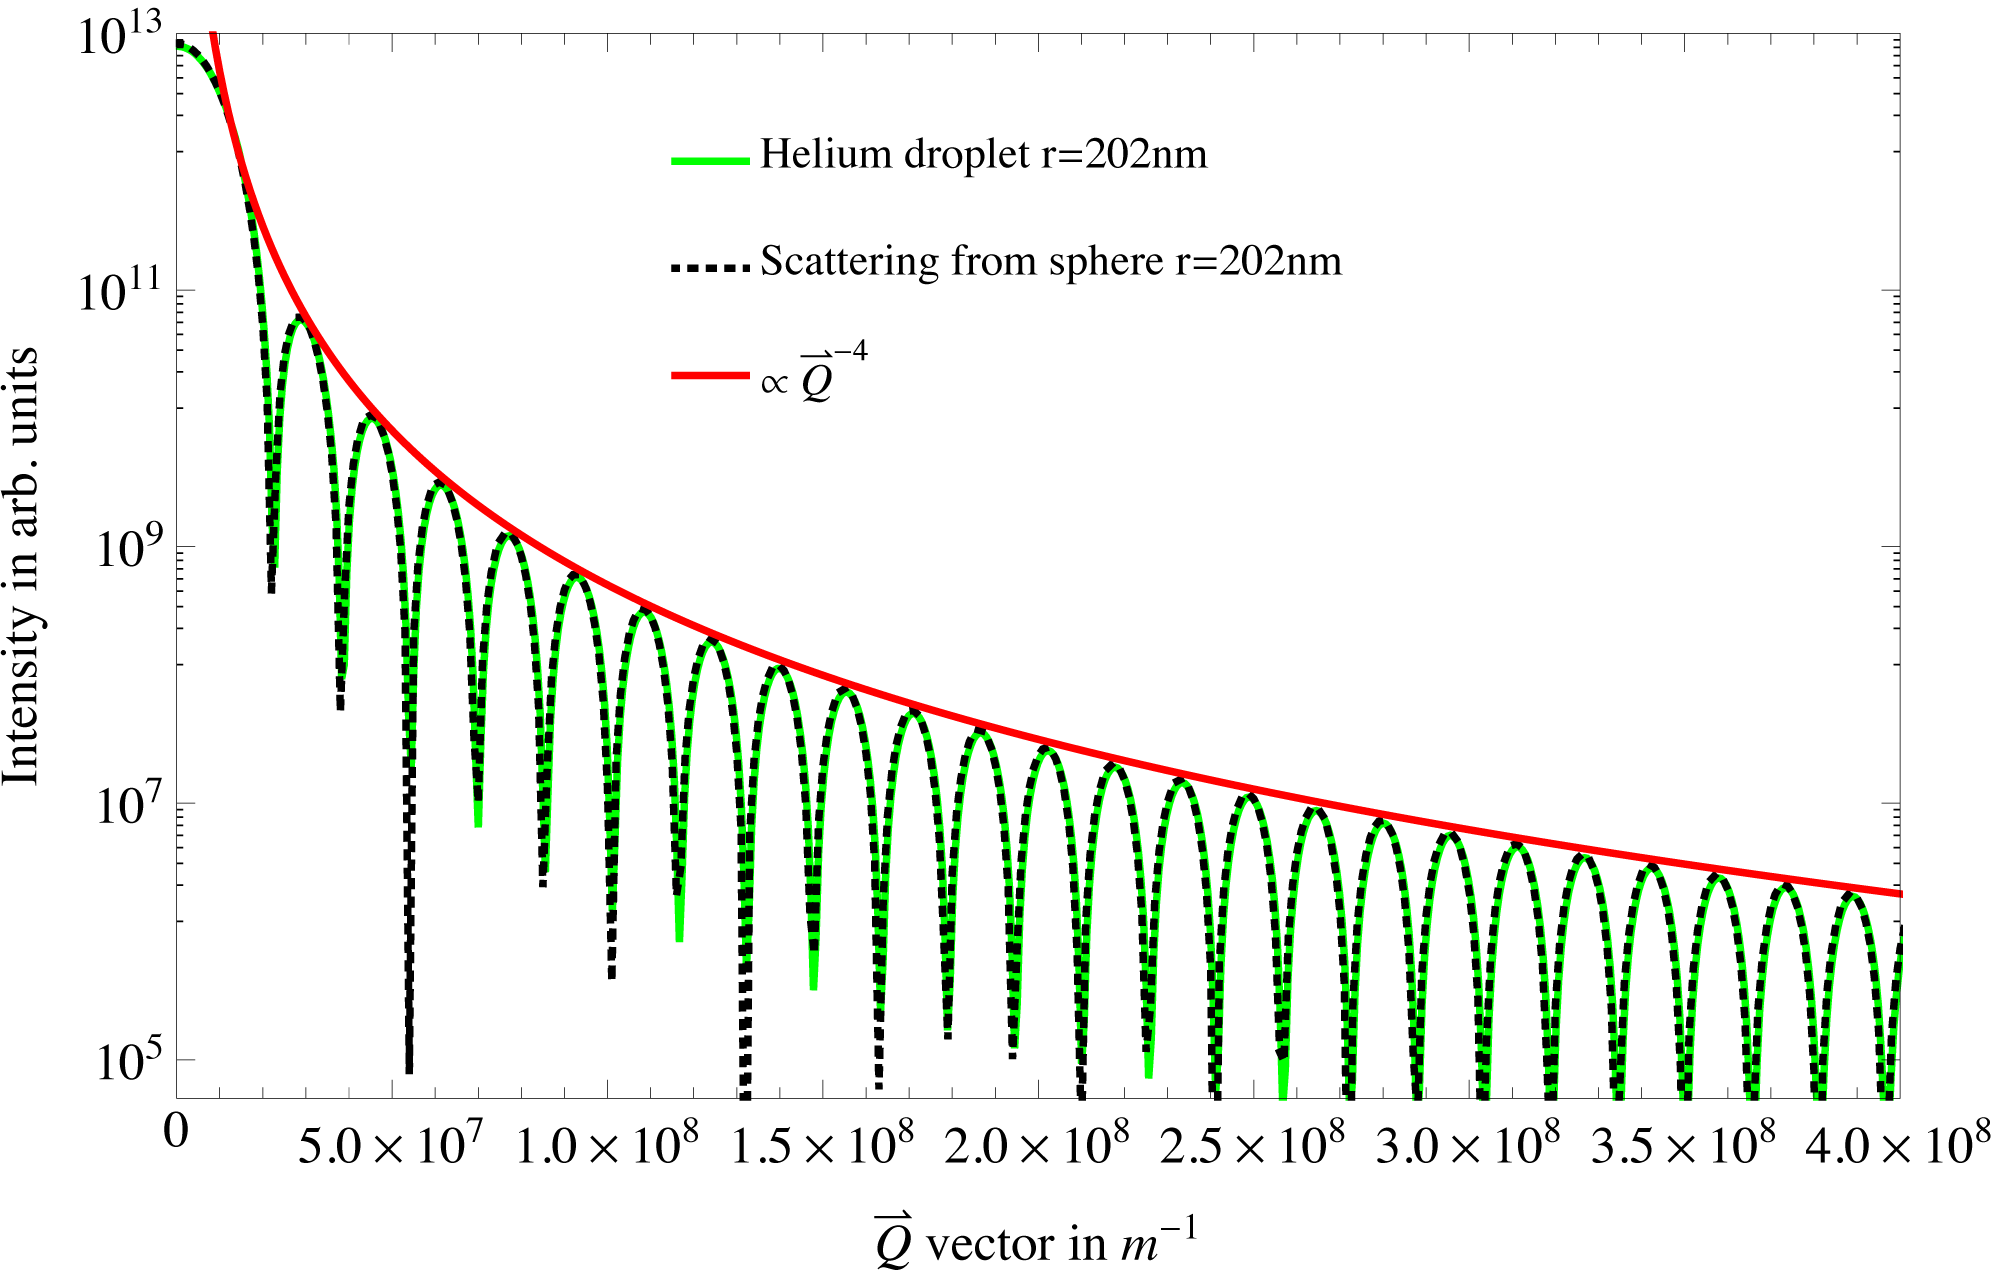
\includegraphics[width=0.80\textwidth]{images/cluster-sphere-intact.png}
	\caption[Comparison of analytical derived scattering and numerical simulations.]{Comparison of analytical scattering from a sphere of radius $R=202$ nm (black curve), Equation \eqref{eq:scattering from sphere}, and scattering of a sphere of radius $R=202$ nm from 2D simulations projected onto 1D (green, dashed curve). The envelope of scattering intensity of a sphere (Porod's law) is $\propto q^{-4}$ (red curve). The analytical scattering and developed simulations agree well with each other.}
	\label{fig:cluster-sphere-intact-2D}
\end{figure}
Figure \ref{fig:cluster-sphere-intact-2D} shows a comparison of the analytical derived scattering of a sphere (see Equation \eqref{eq:scattering from sphere}) with a radius of $r=202nm$ (black, dashed line) and the scattering of the 2D simulations reduced to 1D (green, solid line). The red curve is the envelope of the functions, called Porod's law that scales with $\propto q^{-4}$. The developed simulation agrees well with the analytical scattering, when $k=0$.
%
%
%
\section{Acqiris data sampling considerations}\label{sec:acq-considerations}
%%%%%%%%%%%%%%%%%%%%%%%%%%%%%%
% Adjustments to iTOF data
% - Start value analysis
% - light peak jitter
%%%%%%%%%%%%%%%%%%%%%%%%%%%%%%
\begin{figure}
	\centering
		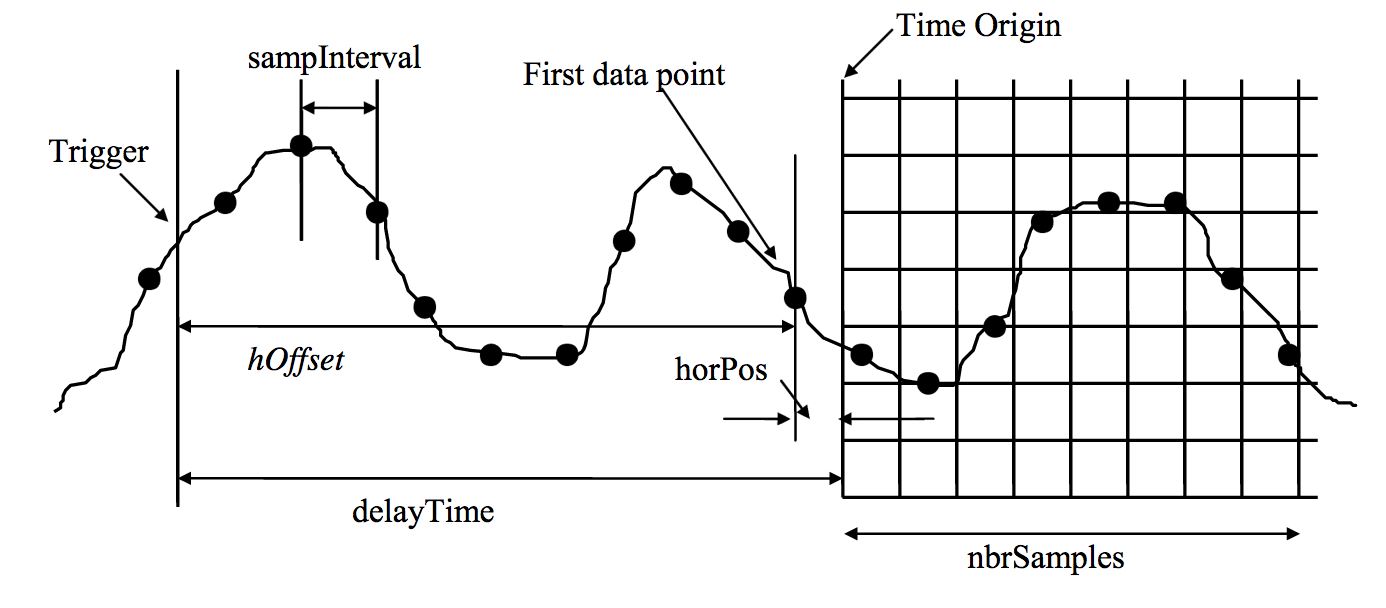
\includegraphics[width=0.49\textwidth]{images/Acqiris-waveform-readout.png}
		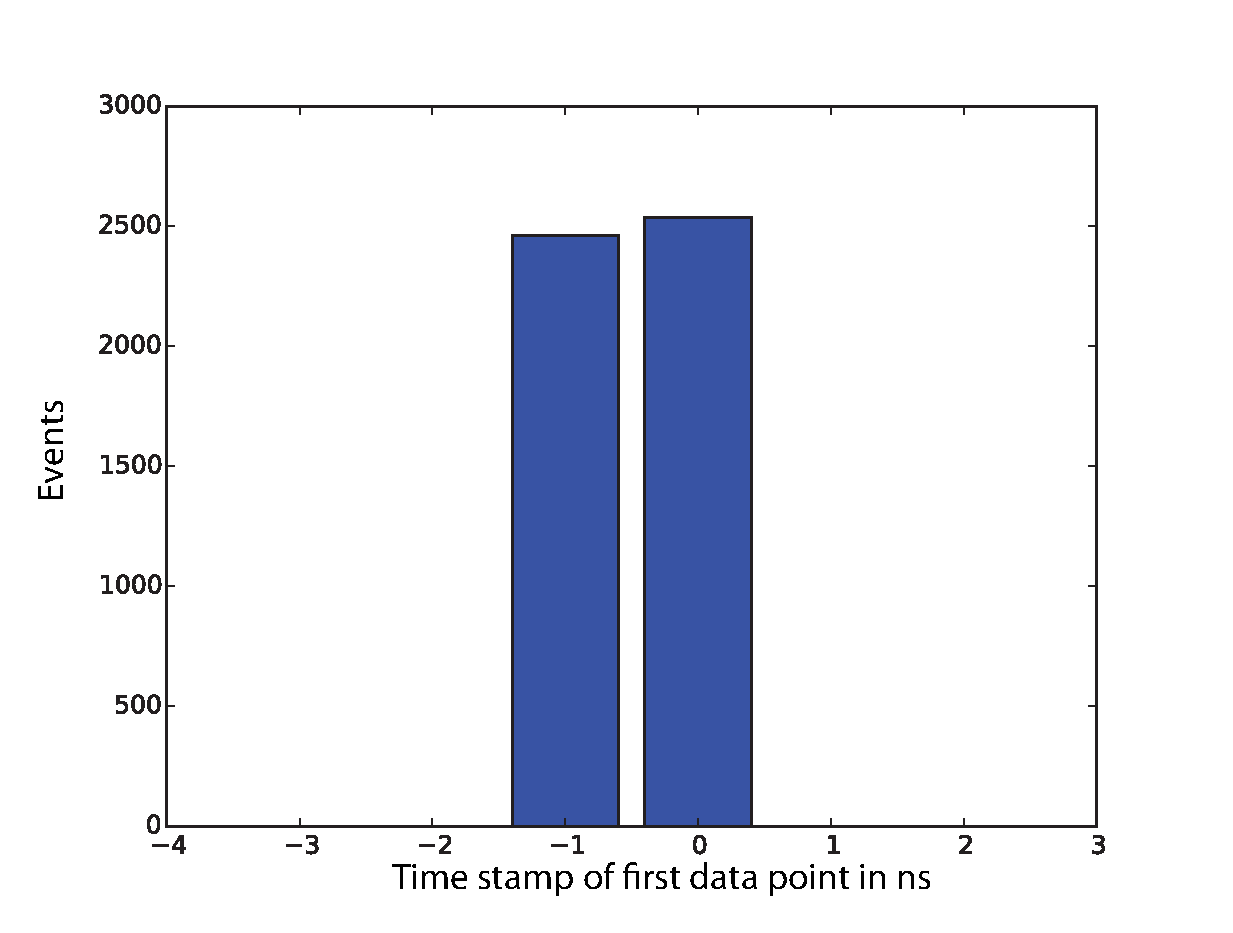
\includegraphics[width=0.49\textwidth]{images/firstDataPoint.eps}
	\caption[First data point in Acqiris sampling.]{Left image from \citep{Acqiris-manual}, it shows the schematics of the timing system in the Acqiris. Due to the finite sampling of the trace, the \textit{first data point} can be before time zero. Right image is a histogram of the the timestamp from the \textit{first data point}.}
	\label{fig:Acqiris-waveform-readout}
\end{figure}
An Acqiris digitizer (now called: Agilent U1065A) has been used to read out the waveform signal from the time-of-flight spectrometer discussed in Section \ref{sec:TOF-spectrometer}. For technical reasons, the Acqiris sampling (internal 'clock') and the electronic trigger (from LCLS EVR) that starts the readout process is generally not in sync. The electronic trigger can occur between sample $\{1,2,..,10\}$. In other words, the Acqiris reads out 40,000 samples but the trigger for the clock comes between sample 0 and 10. As it is illustrated in Chapter \ref{fig:Acqiris-waveform-readout} left, the time difference between the first data point and the time origin is within the sampling interval, thus $\{-1 \text{ns}, 0 \text{ns}\}$, at the sampling rate at 40,000, which is 1 ns per channel \citep{Acqiris-manual}. Figure \ref{fig:Acqiris-waveform-readout} right is an histogram of the First data point timestamp showing the evenly distributed discrepancy. As each read out sample would be different length $\{39991,39992,...,40000\}$, the LCLS DAQ group adds zeros to the end of each array to simplify the analysis of handling arrays of different lengths.\\
\begin{figure}
	\centering
		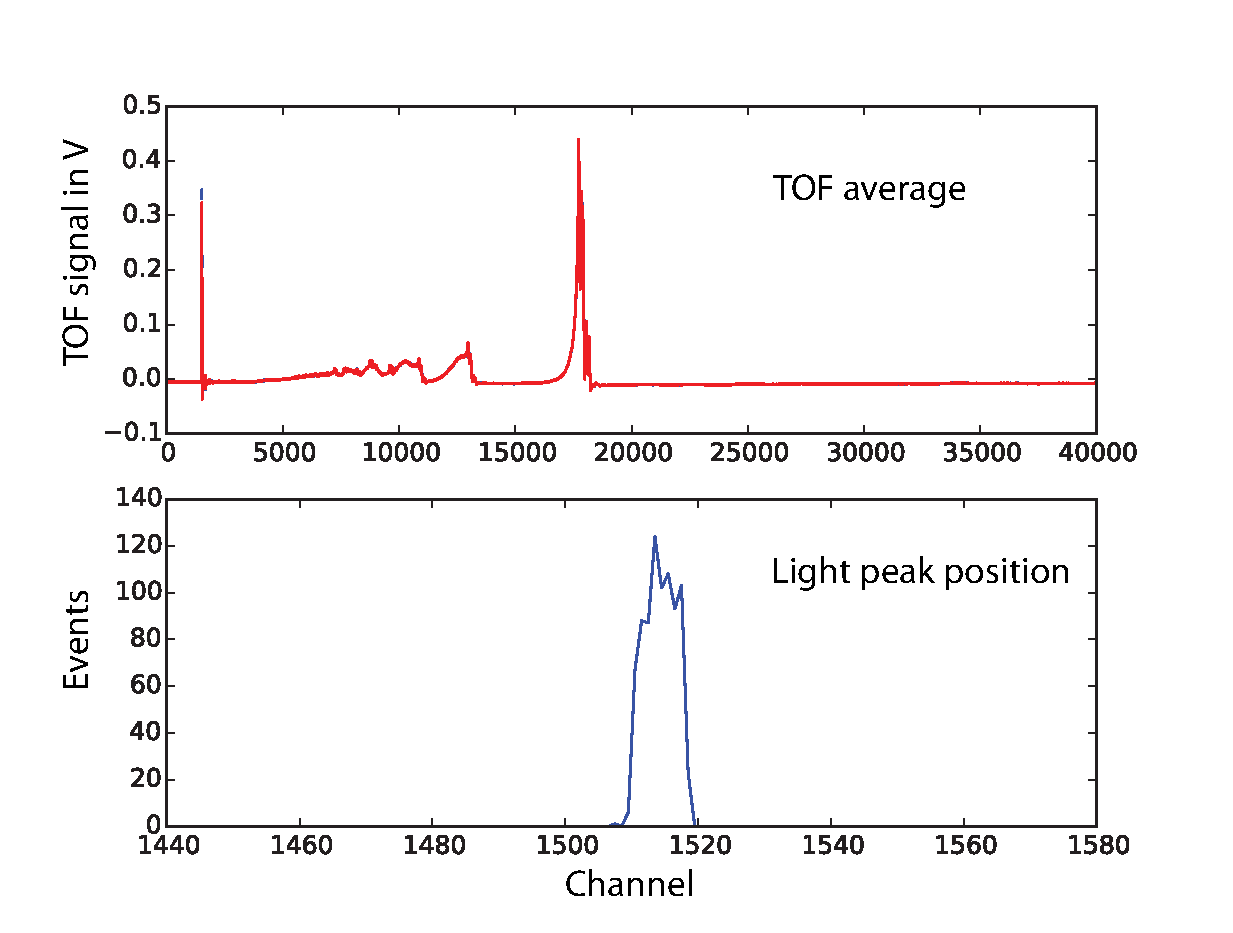
\includegraphics[width=1.00\textwidth]{images/TOF-trace-light-peak.eps}
	\caption[Using light peak to find absolute time zero in Acqiris traces.]{Top plot, average TOF trace of xenon cluster upon irradiation with LCLS. Red curve, corrected run average to account for shifted light peak due to Acqiris sampling. Blue curve, uncorrected average. Bottom image, histogram of light peak channel position ranging between $\sim\pm 5$ of channel 1514.}
	\label{fig:TOF-trace-light-peak}
\end{figure}
However, in an LCLS experiment, the origin of time is best defined by the light peak. The time of flight spectrometer will detect photons scattered of the sample as the pulse is traversing through the system. Figure \ref{fig:TOF-trace-light-peak} bottom shows an analysis of the light peak channel position. The lightpeak occurs within a $\sim10$ ns window and is evenly distributed around channel 1514 due to the Acqiris sampling. Figure \ref{fig:TOF-trace-light-peak} top shows a merely averaged TOF trace (blue curve) and a TOF trace that has been corrected for the light peak occuring at different position (red curve). The LCLS DAQ changes the output of the Acqiris to start with time 0 or -1 and gives out a 40,000 channel long trace by adding zeros for every unsampled channel due to the trigger arrival.\\
The time-of-flight analysis in this thesis accounts for both of these effects and additionally corrects for a common baseline.
%
%
%
\section{Data filtering}\label{sec:hitfinding}
%%%%%%%%%%%%
%- Discuss the hitfinding.\\
%- iTOF vs. pnCCD\\
%- vs. Actual dynamics visible in diffraction images
%%%%%%%%%%%%
\begin{figure}
	\centering
		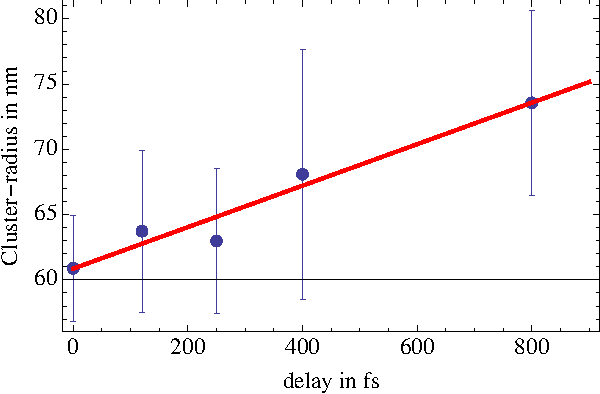
\includegraphics[width=0.49\textwidth]{images/filter-size.pdf}
		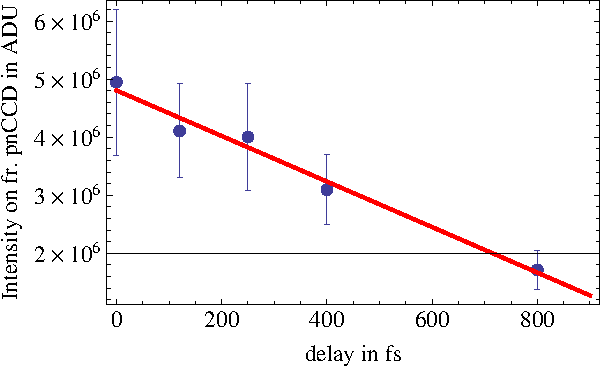
\includegraphics[width=0.50\textwidth]{images/filter-sum-frontpnCCD.pdf}
	\caption[Average cluster size correlated to measured intensity on front pnCCD.]{Left: Average Xenon cluster size of intense hits as a function of pump--probe delay $\Delta t$. Right: Average intensity on the front pnCCD of intense single-shot hits from single Xe-cluster as a function of the pump--probe delay $\Delta t$.}
	\label{fig:filter-size-intensity}
\end{figure}
As described in the above sections, LCLS produces large amounts of data. This data has to be filtered to a point, where it can be used for phase retrieval and plotting. The coincident detection of diffraction image and time of flight trace allow great freedom to filter on useful events. For the present work, a useful event is the interaction of X-ray pump--X-ray probe with a single cluster system. On the one hand, cluster produce the most intense signal on pnCCD and TOF detectors when they are in the center of the intensity profile of the LCLS beam \citep{Gorkhover-2012-PRL}. On the other hand, as the time delay $\Delta t$ of the X-ray pump--X-ray probe is increased, the nanoplasma expansion leads to a decrease in signal on the pnCCD (see Chapter \ref{fig:filter-size-intensity}). This can be extrapolated to an extreme, where cluster would not produce any signal on the front pnCCD. In order to filter on the full bandwidth of interesting hits, a series of filters have been applied. Filtering on ion time of flight high charge states states has been successful in the large scale analysis of events that resolve pump--probe dynamics. In Chapter \ref{fig:filter-size-intensity} left, the xenon pump--probe data has been automatically pre-filtered on xenon ion high-charge states, leaving several thousand events that were then semi-automatically reduced to over 350 single-hit diffraction images. In this semi-automatic process it was determined, whether it was a single hit and the size of a cluster. The size determinations have been performed using the first maxima as described (see Section \ref{sec:saxs}). The plotted events in Chapter \ref{fig:filter-size-intensity} indicate a linear average-Xe-cluster radius increase of $\sim 20\%$ over the course of the first 800 fs (more in Section \ref{sec:xenon-data}). However, to perform phase retrieval and to solve the inverse problem, bright hits containing many photons are required. Therefore, another set of hitfinding has been implemented. This hitfinder determines the scattering intensity of single events automated and the brightest hits that show signs of X-ray induced dynamics have been selected semi-automated. These hits undergo a phase retrieval to reveal their electron density. To clarify, single He- and Xe-cluster hits show X-ray induced dynamics, when the 1d reduction of the intensity profile differs from the scattering of an intact sphere, i.e., $\tfrac{I}{F_{\text{intact}}^{2}} \ll 1$. The case of X-ray induced dyanmics in HeXe-cluster is discussed in more detail in Section \ref{sec:helium-xenon-data}.
%
%
%